\section{Molekularna verižnica} 
Definaramo energijsko funkcijo diskretnih točk v verižnici
\begin{equation}
    E = \sum_{i=1}^{N} \alpha \, h_i + \sum_{i=1}^{N-1} 0,5\, (h_{i+1}-h_i)^2
\end{equation}
kjer $\alpha$ predstavlja potencial za gravitacijsko energijo in druga vsota prožnostno energijo med dvema sosednjim členoma. V Metropolisovem algoritmu premikamo naključne člene v verižnici za en člen navzgor ali navzdol naključno. Pri tem uvedemo omejitev za največni poves 18, saj obstaja 19 energijskih nivojev in 17 diskretnih točk. V algoritmu z iterativnim reševanjem iščemo minimum dane energijske funkcije. Pri tem sprejmemo tako vse rešitve, ki zadostijo pogoju zmanjšanja celokopne energije, kot tudi tiste, ki tem pogoji ne zadostijo, vendar je naključno generirano število $\mathcal{A}$ na uniformnem intervalu [0,1) manjše od:
\begin{equation}
    \mathcal{A} < e^{-\beta\,\Delta E}
\end{equation}
Tako $\beta$ predstavlja obratno vrednost temperature in togosti (podajnost) povezav med delčki verižnice $k^{-1}T^{-1}$.

Na spodnjih sklikah je prikazano, kako konvergira rešitev tekom iteracij algoritma za verižnico, omejeno na 19 energijskih nivojev in neomejeno, ko mejo limitiramo v $\infty$. 

V začetnih nekaj 100 iteracijah skoraj ni sprememb energije; to je tako zvani ``burn in'' in je v našem primeru vidno le na log skali. Nato začne rešitev konvergirati, kar je tudi grafično dobro vidno iz lege členov verižnice glede na ravnovesno lego, izračunano po paraboli oblike $f(x) = a\,x^2 + b\,x+c$. Ko algoritem doseže minimalno energijo, se ustali, možne so le še oscilacije nad ravnovesno (minimalno) lege, na katere, tako kot na dolžino ``burn in'' območja, najodločilneje vpliva koeficient $\beta$.
\begin{figure}[ht]
    \centering
    \begin{minipage}{0.49\textwidth}
        \centering
        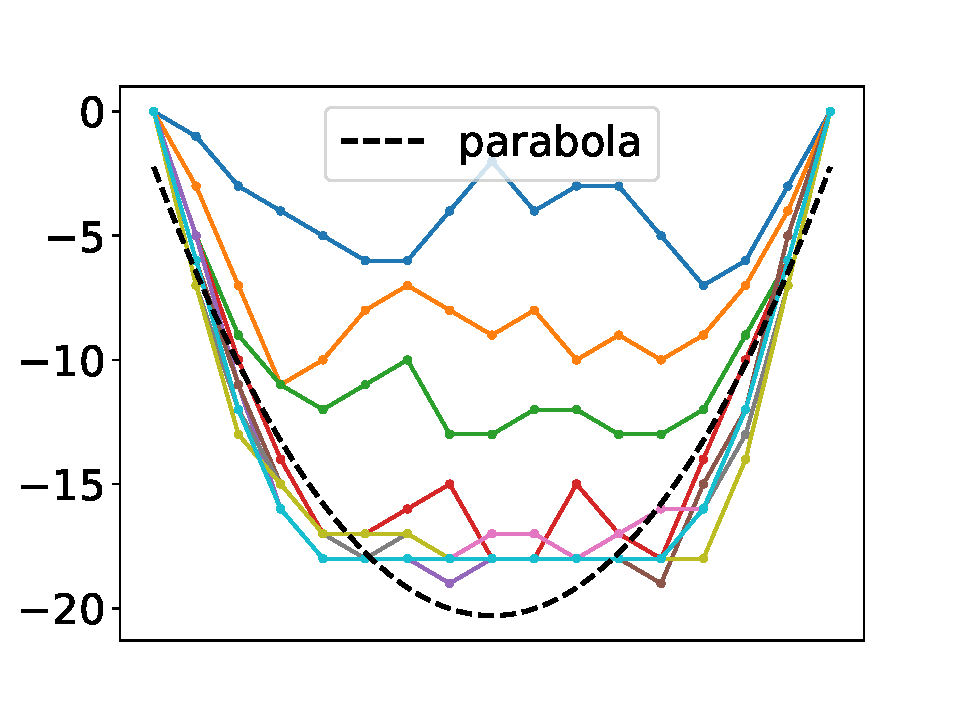
\includegraphics[width=\linewidth]{8.nal slike/konvergenca_metropolis_omejen.pdf}
        \caption{Konvergenca Metropolisovega algoritma pri omejeni verižnici}
    \end{minipage}
    \begin{minipage}{0.49\textwidth}
        \centering
        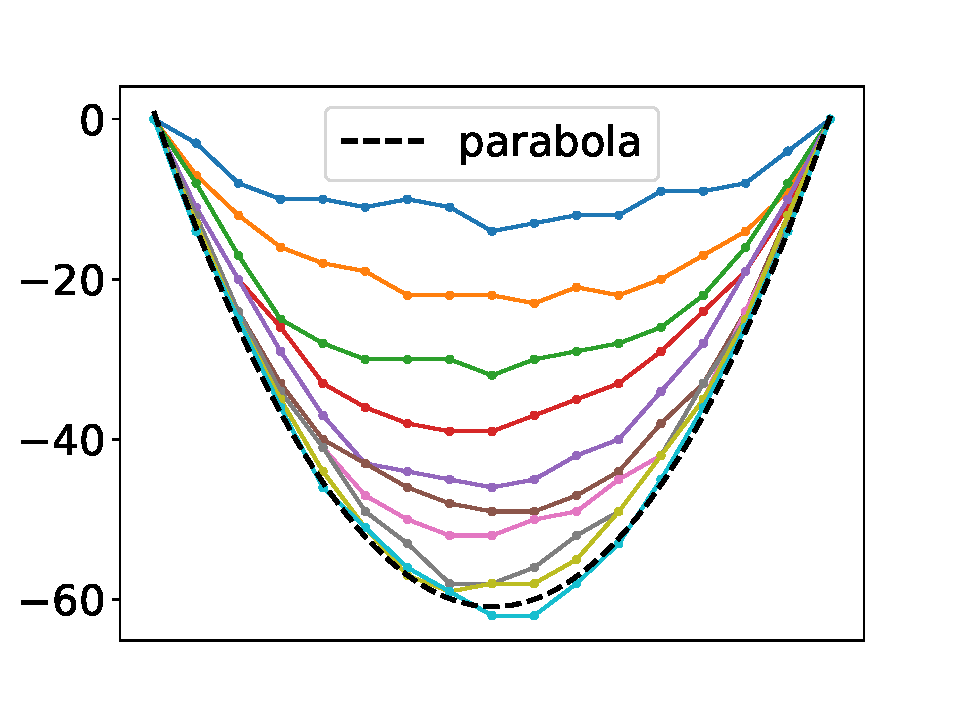
\includegraphics[width=\linewidth]{8.nal slike/konvergenca_metropolis.pdf}
        \caption{Konvergenca Metropolisovega algoritma pri neomejeni verižnici}
    \end{minipage}
\end{figure}

Pričakovano, nižanje koeficienta $\beta$, torej višanje temperature, povzroča večja nihanja energije tako v omejeni, kot neomejeni verižnici. Zanimivo in hkrati nepojasnjeno pa je to, da se pri tem nekoliko spremeni tudi ravnovesna lega, vendar je mogoče, da bi se pri večjem številu iteracij poravnale. Tega mi nismo poizkušali.

Zanimiva je tudi razlika med številom iteracij omejene in neomejene verižnice, pri kateri prihaja do ravnovesne lege. Ta je povezana z omejitvijo -- ravnovesno energijo, in bo pojasnjena v sledečem.
\begin{figure}[ht]
    \centering
    \begin{minipage}{0.49\textwidth}
        \centering
        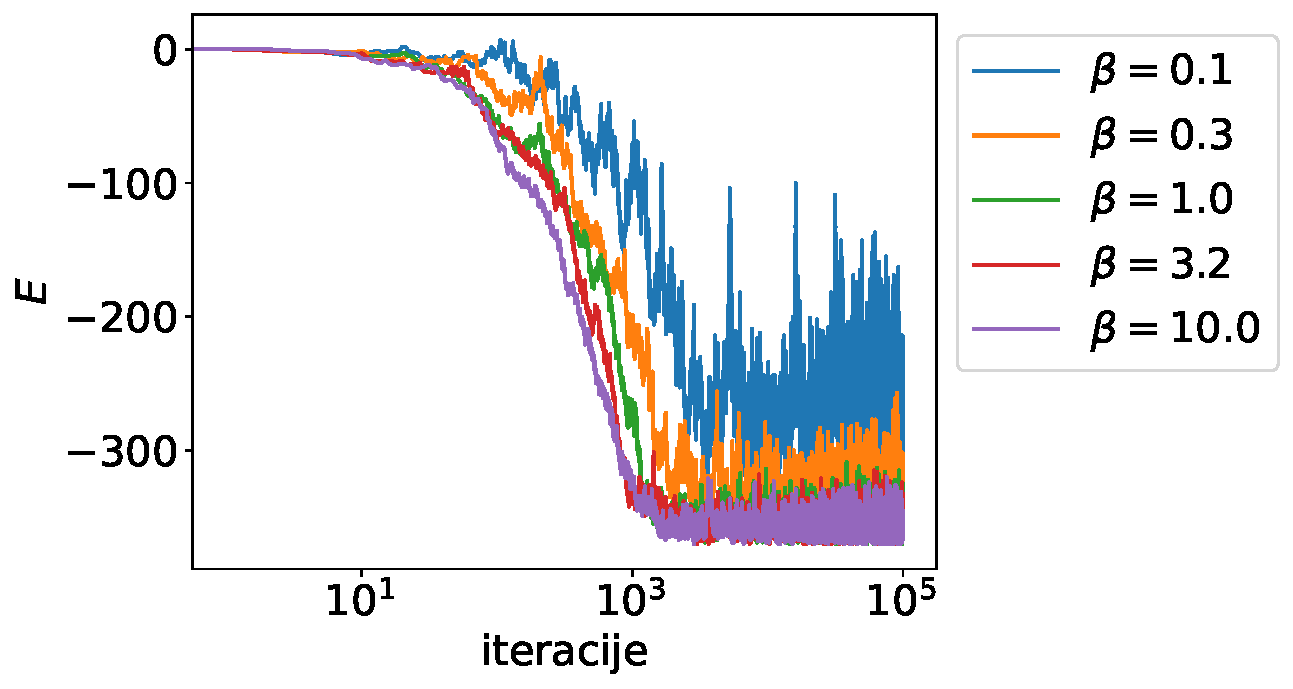
\includegraphics[width=\linewidth]{8.nal slike/vpliv_beta_omejeno.pdf}
        \caption{Vpliv temperature na omejeno verižnico pri $\alpha = 2$}
    \end{minipage}
    \begin{minipage}{0.49\textwidth}
        \centering
        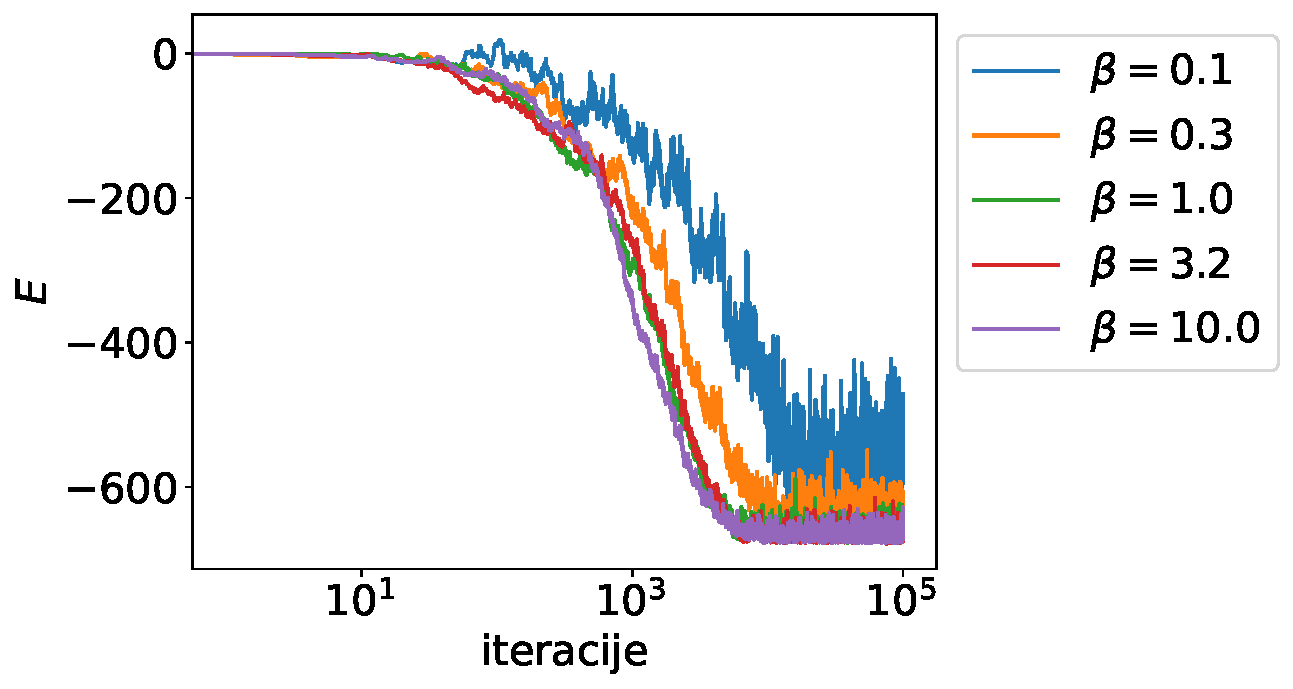
\includegraphics[width=\linewidth]{8.nal slike/vpliv_beta_neomejeno.pdf}
        \caption{Vpliv temperature na neomejeno verižnico pri $\alpha = 2$}
    \end{minipage}
\end{figure}

Spreminjamo lahko tudi potencial gravitacijske energije $\alpha$, kar sicer ni fizikalno smiselno, vendar tako lahko npr. občudujemo rezultate v različnih gravitacijskih poljih. To rezultira v pričakovanih spremembah ravnovesnih leg in bistveno ne vpliva na oscilacije (izgledajo majše le zaradi skaliranja!) in iteracije do dosega ravnoverne lege.

Podoben vpliv ima tudi omejitev verižnice z končnim številom energijskih nivojev $h_{\text{max}}$, vendar tukaj prihaja tudi do spremembe števila potrebnih iteracij do ravnovesne lege. To se godi zaradi spremembe velikosti ravnovesne enrgije -- več nivojev, višja energija -- in enake konvergence algoritma. Pri tem velja poudariti, da omejitev $h_{\text{max}} =100$ že predstavlja ravnovesno lego, saj se naša verižnica s 17 členi globlje ne povesi.
\begin{figure}[ht]
    \centering
    \begin{minipage}{0.49\textwidth}
        \centering
        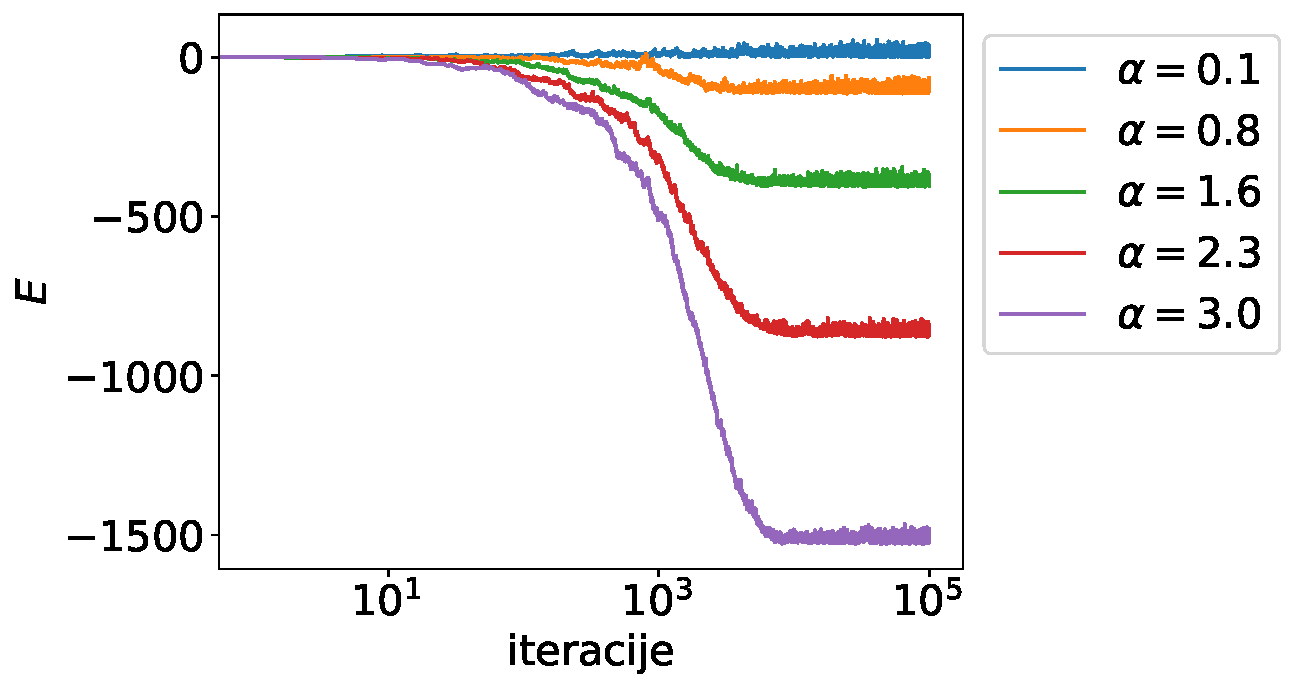
\includegraphics[width=\linewidth]{8.nal slike/vpliv_alpha.pdf}
        \caption{Vpliv $\alpha$ na neomejeno verižnico pri $\beta = 1$}
    \end{minipage}
    \begin{minipage}{0.49\textwidth}
        \centering
        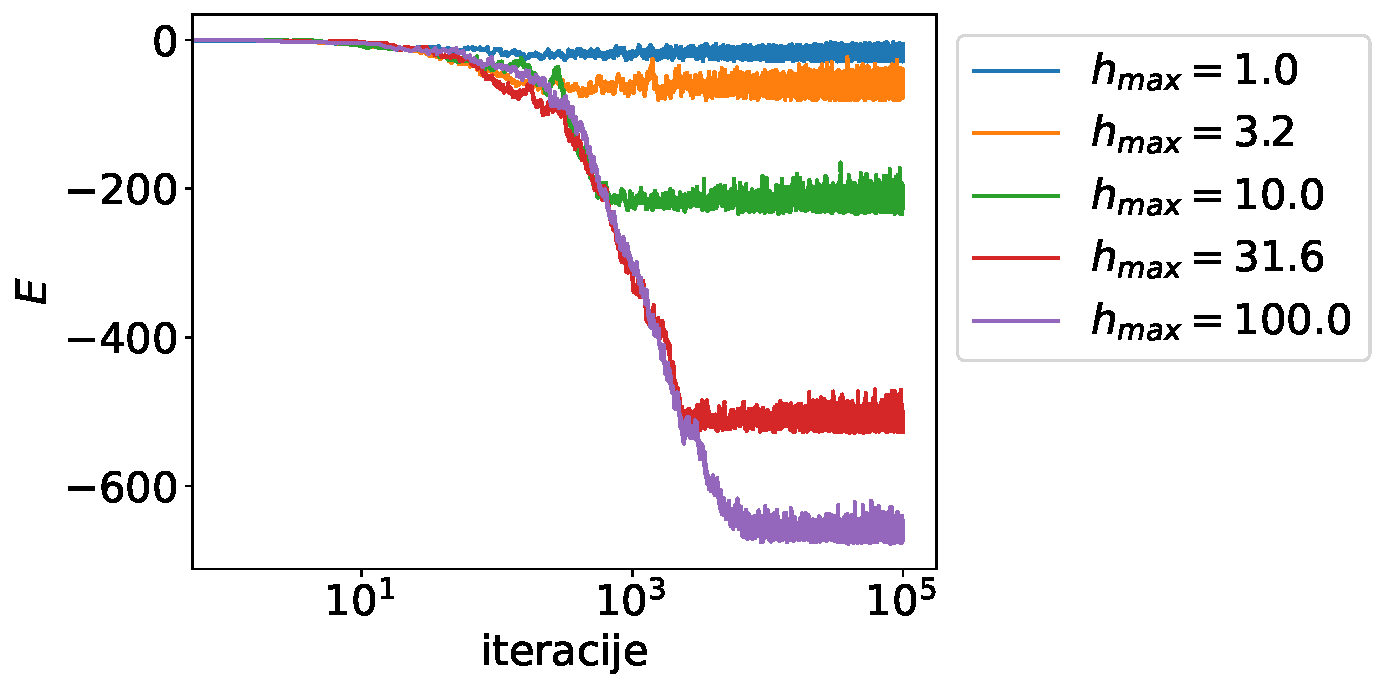
\includegraphics[width=\linewidth]{8.nal slike/vpliv_h_max.pdf}
        \caption{Vpliv največjega možnega povesa omejene verižnice $h_{\text{max}}$ pri $\alpha = 2$, $\beta =1$}
    \end{minipage}
\end{figure}

Ker so do sedaj bila začetna stanja verižnice do sedaj vedno enaka nič, smo poizkusili, kako začetno stanje verižnice vpliva na rezultat. Ugotovljeno je, da začetno stanje presenetljivo vpliva na ravnovesno energijo in ravnovesno stanje, kar prikazuje spodnja slika, kjer se očitno razlikujejo ravnovesne lege od ravnovesne lege ničelnega začetnega stanja. To ni le posledica oscilacij algoritma.
\begin{figure}[H]
    \centering
    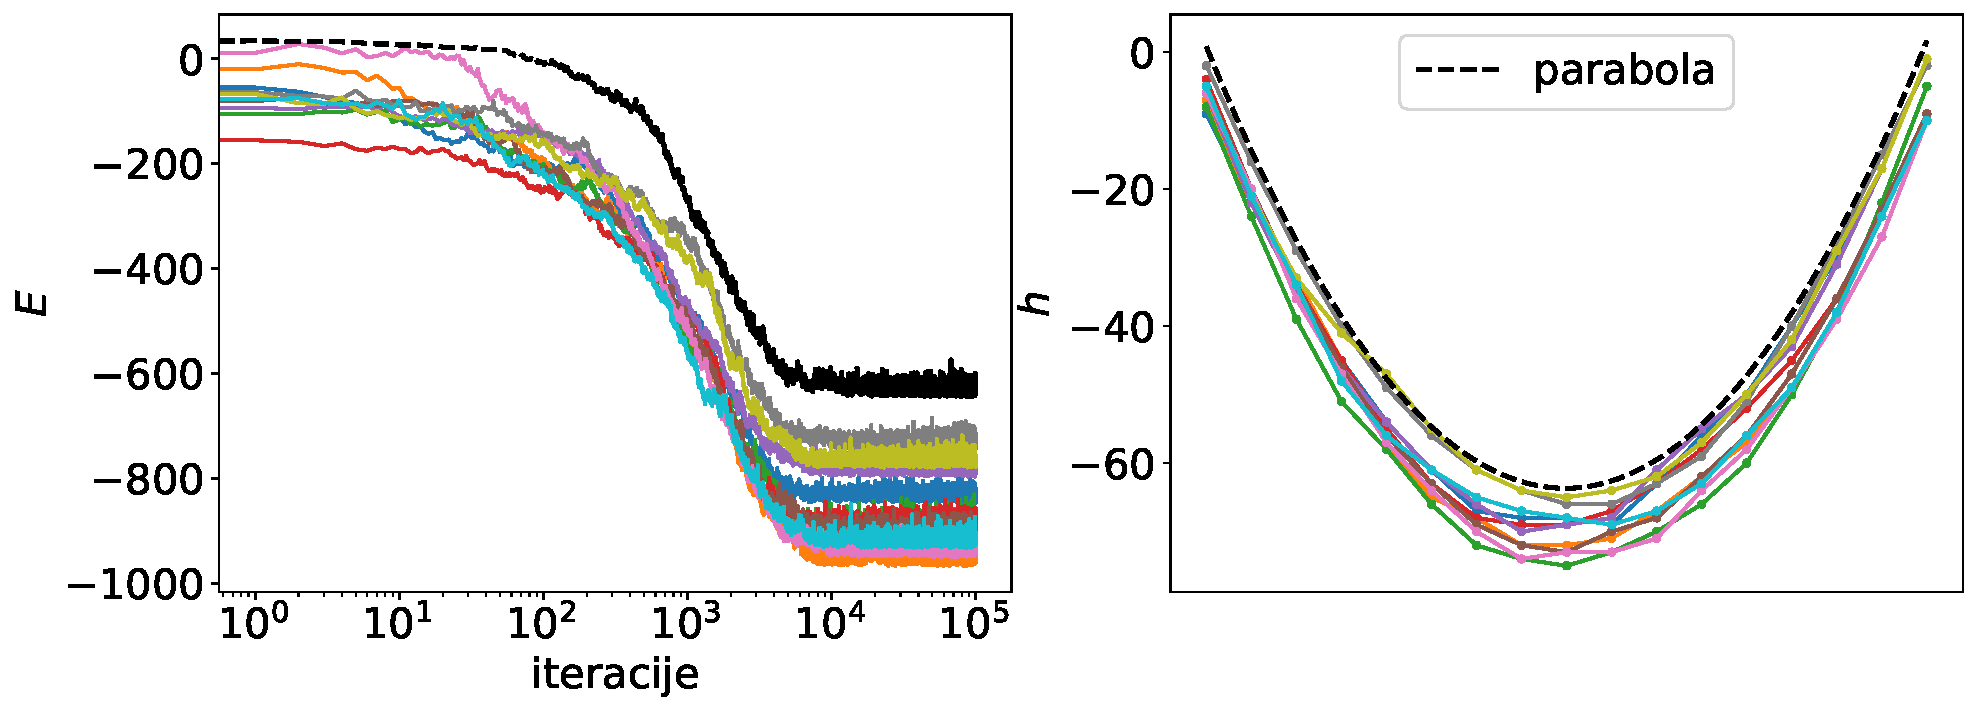
\includegraphics[width=\linewidth]{8.nal slike/vpliv_začetka.pdf}
    \caption{Vpliv začetnih pogojev, naključno razporejenih med 0 in -10. Parabola predstavlja ravnovesno lego verižnice z vsemi začetnimi stanji, enakimi nič. $\alpha = 2$, $\beta =1$}
\end{figure}

Dalje smo si drznili spremeniti tudi število delcev v neomejeni verižnici. Kot posledica sta nastala spodnja dva grafa, kjer vidimo, da število členov bistveno vpliva na ravnovesno energijo in čas, potreben do ustaljenega stanja. Ker moramo tako izvesti različno število iteracij, glede na število členov ($n$), smo izvedni adaptivno število iteracij oblike $1000\,n^{1,5}$, kar je ustrezno, glede na sliko \ref{fig:delci_1}. Tukaj lahko tudi vizualno določimo mejo ustaljenega stanja kot linearno funkcijo $E_u(x) = -x/10$, kjer je x število iteracij. Prav tako izgleda iz potekov verižnic lepo popisljiv potek lege največjega povesa:
\begin{equation}
    \begin{pmatrix}
        x \\ h_{\text{max}}
    \end{pmatrix}
    =
    \begin{pmatrix}
        \frac{n}{2} \\ -\frac{a\, n^2}{4}
    \end{pmatrix}
\end{equation}
kjer smo določili koeficient parabole $a$ iz zadnjega izračuna (največ členov). Predpis funkcije je viden na grafu, vendar je moč opaziti, da se za večja števila členov ne prilega povsod tako lepo. Na sliki \ref{fig:delci_2} je to že vidno, prav tako se je pri velikem številu členov močno povečalo potrebno število iteracij, ki jih naš algoritem ni izvedel, vendar verižnica ne izgleda deformirano, zato napaka ni velika. Prav tako je premica, ki popisuje ustaljeno stanje empirična in nujno ne opisuje ustaljenega stanja zadovoljivo v vseh primerih.
\begin{figure}[ht]
    \centering
    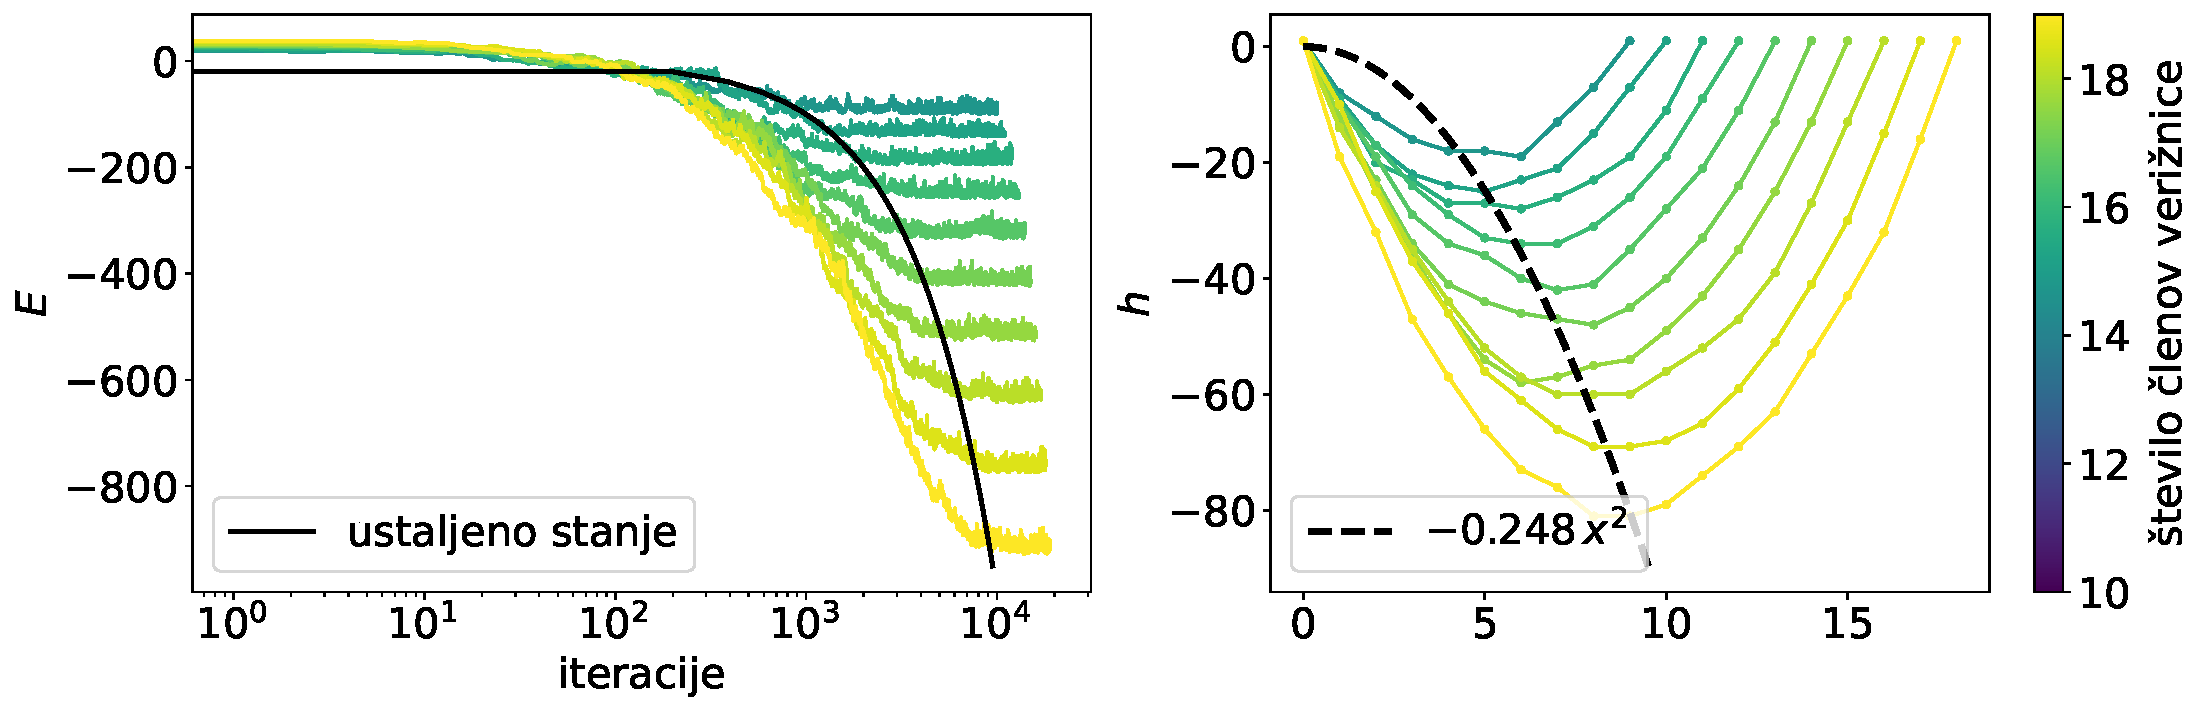
\includegraphics[width=\linewidth]{8.nal slike/vpliv_dolžine.pdf}
    \caption{Vpliv števila delcev v neomejeni verižnici na ravnovesno energijo pri $\alpha = 2$, $\beta =1$}
    \label{fig:delci_1}
\end{figure}
\begin{figure}[H]
    \centering
    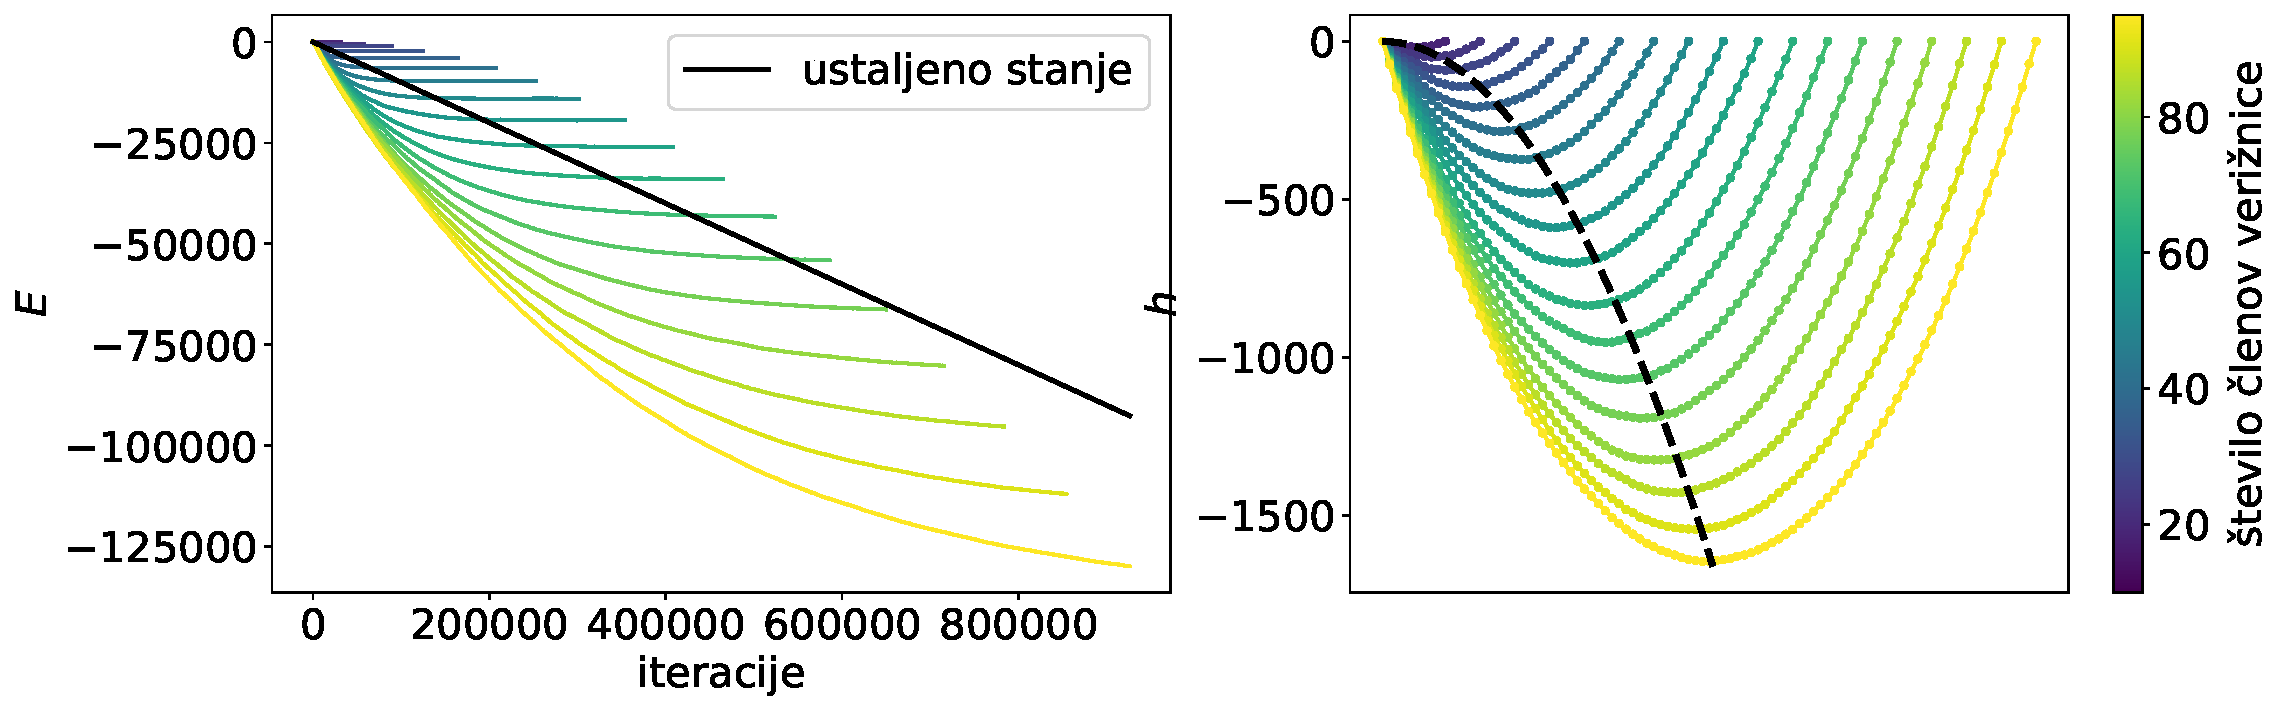
\includegraphics[width=\linewidth]{8.nal slike/vpliv_dolžine_več.pdf}
    \caption{Potrebno število iteracij algoritma narašča z večanjem števila členov}
    \label{fig:delci_2}
\end{figure}

Tekom izračuna zgornjega grafa smo beležili tudi uspešne (in neuspešne iteracije), ko pride do spremembe enega energijskega nivoja, ki so prikazane na spodnjem grafu. Nihanje vrednosti je zaradi naključnosti algoritma pričakovano, prav tako tudi trend upadanja deleža sprejetih potez zaradi večjega števila točk. Iz deleža lahko tudi sklepamo o dolžini trajanja in konvergenci algoritma.
\begin{figure}[ht]
    \centering
    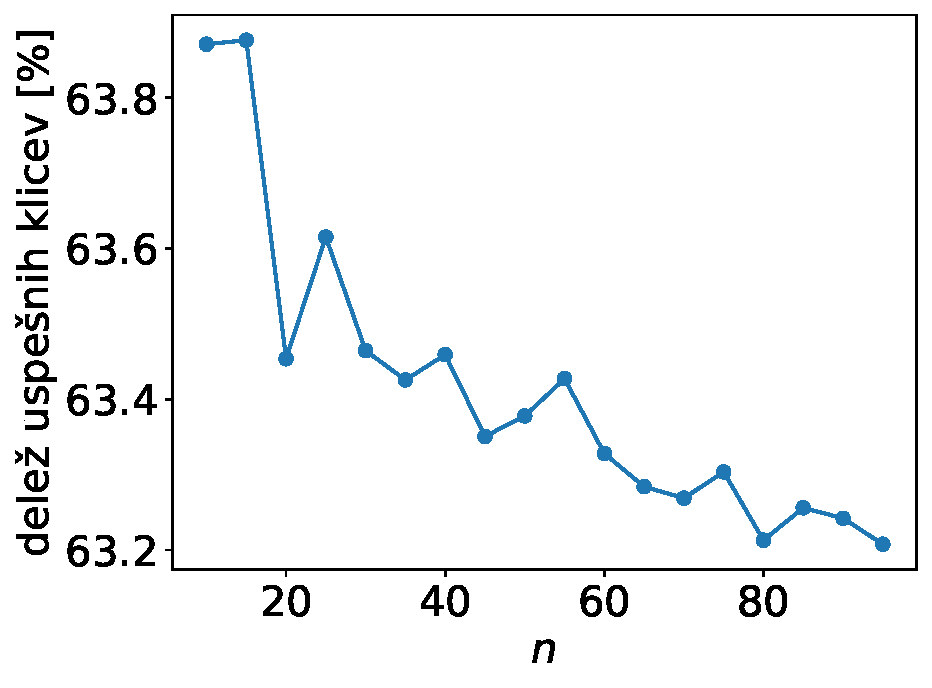
\includegraphics[width=0.38\linewidth]{8.nal slike/delež klicev_n.pdf}
    \caption{Delež sprejetih potez v algoritmu pri neomejeni verižnici in $\alpha = 2$, $\beta =1$}
\end{figure}

\section[]{Isingov model}
\setcounter{figure}{0}
Uporabili smo opis magnetnega stanja snovi s Hamiltonovim operatorjem, podanim v navodilu vaje. V izogib vsakokretnemu izračunu celotne skupne energije računamo le spremembo, potrebno za odločitev po Metropolisu:
\begin{equation}
    \Delta E = -2\,J\,S_{i,j}\,(S_{i-1,j}+S_{i+1,j}+S_{i,j-1}+S_{i,j+1})+2\,H\,S_{i,j}
\end{equation}

Izvedli smo simulacijo stanja po 200 000 iteracijah za primer periodičnih in neperiodičnih robnih pogojev. Snov je feromagnetna $J=1$ in ni v zunanjem magnetnem polju $H=0$. Opazimo, da na magnetizacijo močno vpliva temperatura. Prav tako obstaja tudi odstopanje glede na različna robna pogoja, saj pri perodičnim zvezno prehajamo preko roba, zato je tam lepši potek, čerprav se energija bistveno ne razlikuje. Uporabljali bomo periodičnega, saj pri majšem številu elementov to lahko močneje vpliva na potek energije.
\begin{figure}[ht]
    \centering
    \begin{minipage}{0.49\textwidth}
        \centering
        \includegraphics[width=\linewidth]{8.nal slike/metopolis_T_0.1.pdf}
        \caption[short]{$T=0.1$°C}
    \end{minipage}
    \begin{minipage}{0.49\textwidth}
        \centering
        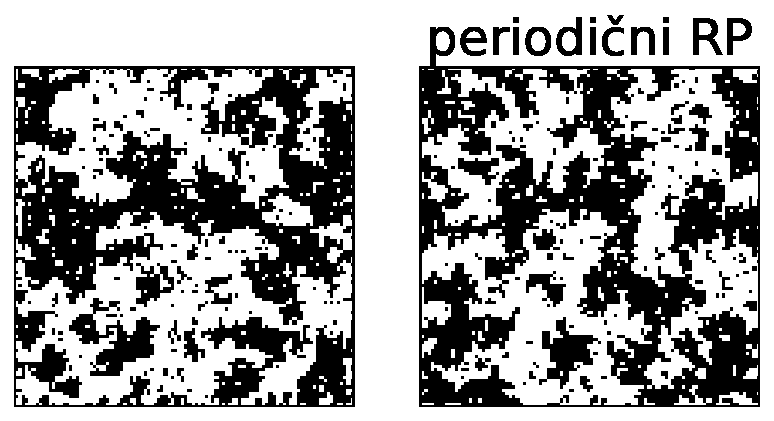
\includegraphics[width=\linewidth]{8.nal slike/metopolis_T_2.27.pdf}
        \caption[short]{$T=T_C=2.27$°C}
    \end{minipage}
    \begin{minipage}{0.49\textwidth}
        \centering
        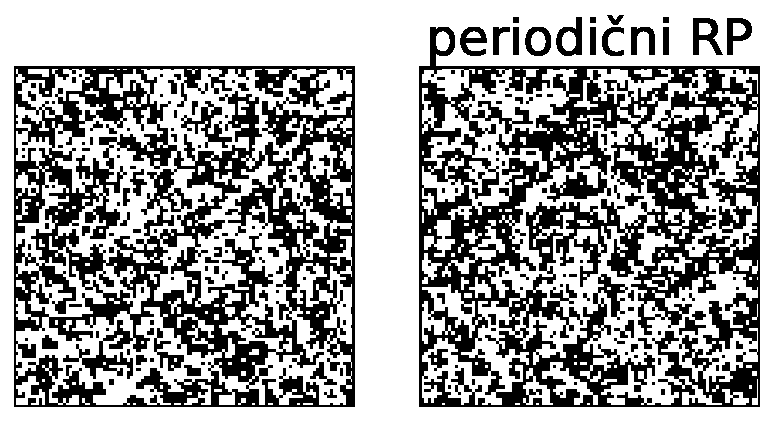
\includegraphics[width=\linewidth]{8.nal slike/metopolis_T_4.pdf}
        \caption[short]{$T=4.0$°C}
    \end{minipage}
    \begin{minipage}{0.49\textwidth}
        \centering
        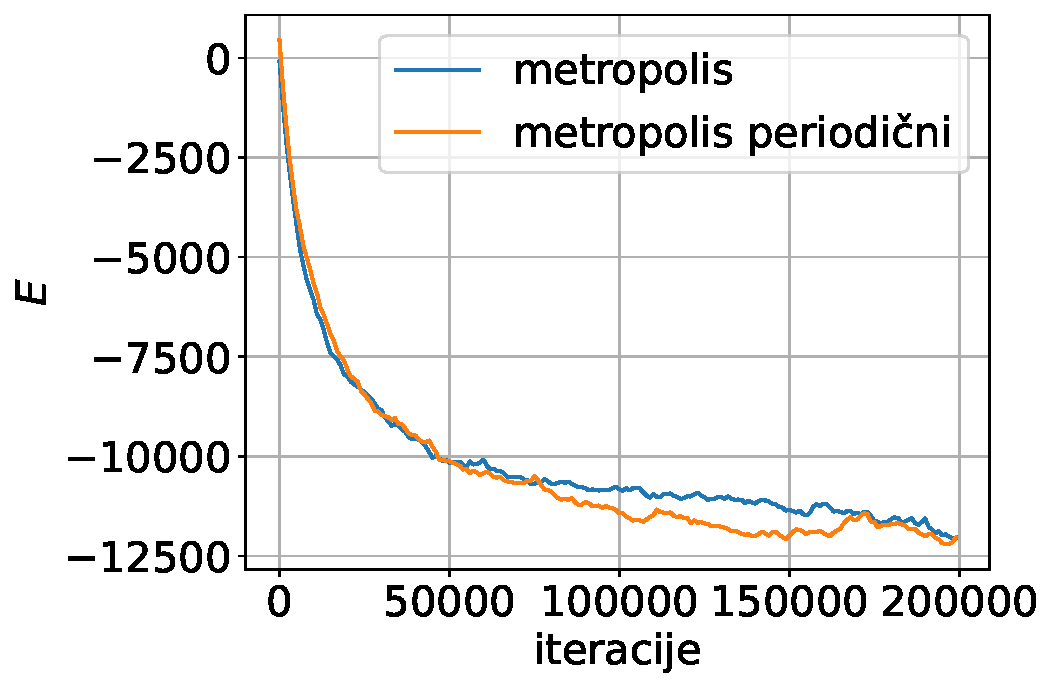
\includegraphics[width=\linewidth]{8.nal slike/metopolis_potek_E.pdf}
        \caption[short]{potek energije pri $T=2.27$°C}
    \end{minipage}
\end{figure}

Na sliki \ref{fig:fp_polje} je prikazana odvisnost magnetizacije glede na različne temperature. Z navpično črto je označena toretično izračunana temperatura faznega prehoda $T_{fc}=2.27 J/k_B$, ki pa velja le za odsotnost zunanjega magnetnega polja. Predvsem pri vrednosti T blizu 0 je moč večja nihanja opaziti, navkljub povprečenju. To lahko izboljšamo z večjo mrežo in več iteracijami, da zagotovimo fazni prehod do konca, vendar to terja večji računski čas, zato so odvisnosti od števila delcev prikazani na slikah \ref{fig:fp_mreža} in \ref{fig:fp_mreža_H}. Vidimo, da velikost mreže očitno izboljša rešitev v zunanjem polju, vendar tam teoretična temperatura $T_{fc}$ ne velja več, pri primeru brez polja pa bi morali povečati število iteracij, saj izgleda da rešitev še ni ustaljena.
\begin{figure}[H]
    \centering
    \begin{minipage}{0.49\textwidth}
        \centering
        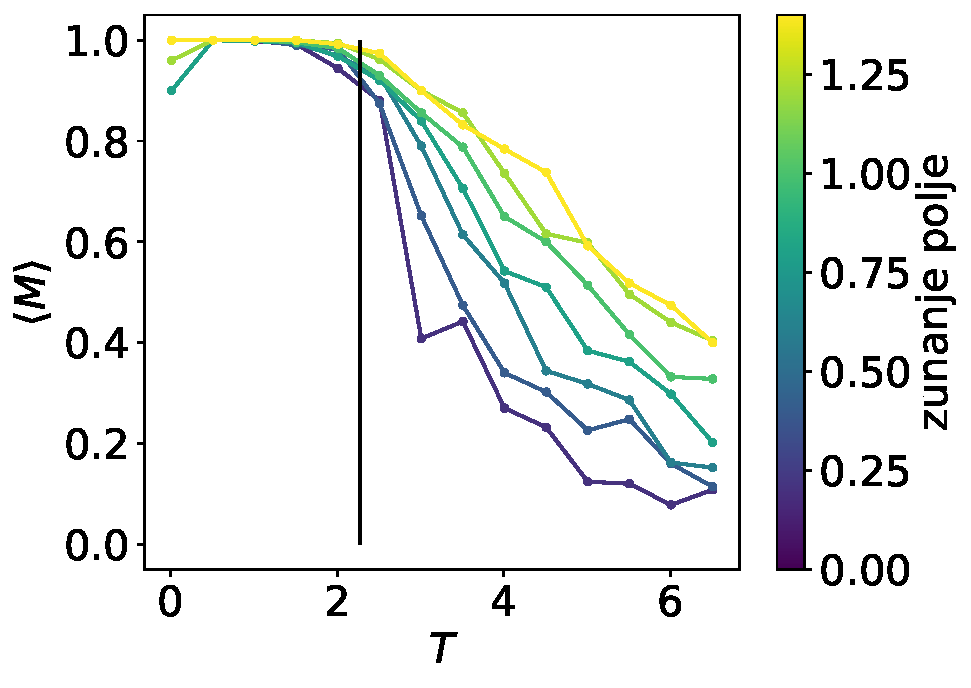
\includegraphics[width=\linewidth]{8.nal slike/vpliv_H_magnetizacija.pdf}
        \caption[short]{Vpliv zunanjega polja na fazni prehod pri 10 ponovitev na mreži 10x10 v 10000 iteracijah}
        \label{fig:fp_polje}
    \end{minipage}
    \begin{minipage}{0.49\textwidth}
        \centering
        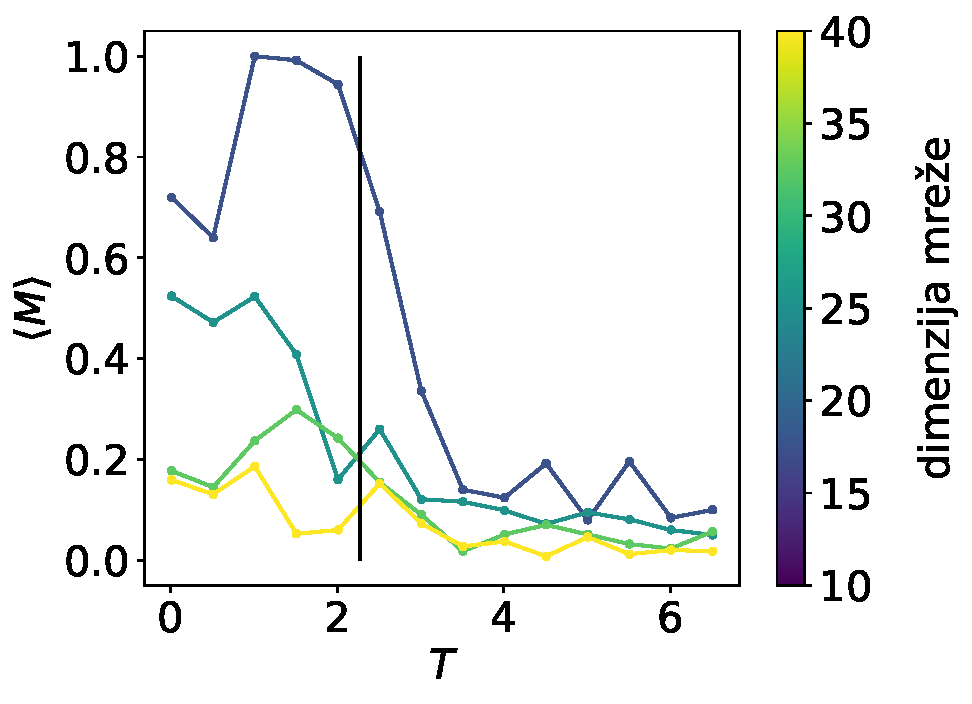
\includegraphics[width=\linewidth]{8.nal slike/vpliv_n_magnetizacija.pdf}
        \caption[short]{Vpliv velikosti mreže na fazni prehod pri 5 ponovitev v 10000 iteracijah brez zunanjega polja}
        \label{fig:fp_mreža}
    \end{minipage}
    \begin{minipage}{0.49\textwidth}
        \centering
        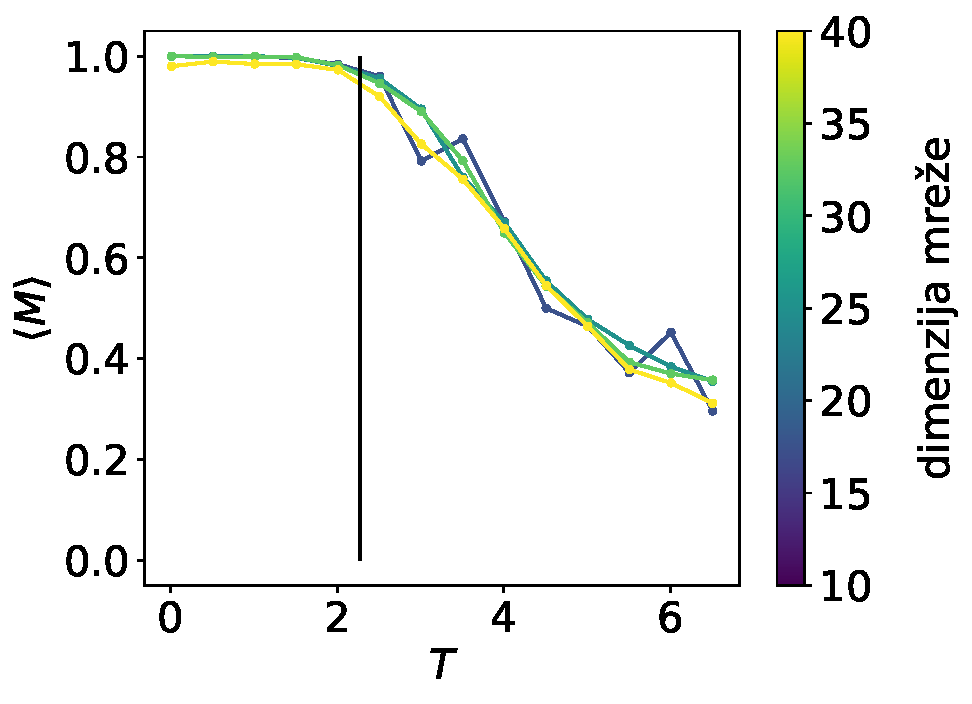
\includegraphics[width=\linewidth]{8.nal slike/vpliv_n_magnetizacija_H1.pdf}
        \caption[short]{Vpliv velikosti mreže na fazni prehod pri 5 ponovitev v 10000 iteracijah z zunanjim poljem $H=1$}
        \label{fig:fp_mreža_H}
    \end{minipage}
\end{figure}

Sedaj pogledamo še, kako poteka energija v odvisnosti od temperature \ref{fig:E1} in zunanjega magnetnega polja \ref{fig:E2}. Oba izračuna sta izvedena za feromagneten material v domeni 100x100. Ker sistemi z višjim zunanjim poljem prej dosežejo ravnovesje, v sledeče računamo v $H=0,5$. Opazimo, da prihaja pri višjih temperaturah do večjih oscilacij, vendar se sistem, čeprav ima višjo ravnovesno energijo ne stabilizira hitreje.

Na sliki \ref{fig:E3} je prikazano, kako je porazdeljena energija tekom celotne simulacije, prav tako je za ravnovesno izbrana energija z najmanjšo vrednostjo, ki je večkrat dosežena pri nižjih tempereaturah, zaradi manj oscilacij.

Slika \ref{fig:E4} prikazuje, kako povprečna ravnovesna energija zavisi od temperature. Pričakovali smo naraščajočo krivuljo, vendar ne takšne, ki izgleda podobna obratnem poteku magnetizacije v prejšnjem skopu. Prav tako lahko tukaj začuda opazimmo odvisnost od teoretične temperature faznega prehoda, čeprav smo  računali v magnetnom polju $H=0,5$.
\begin{figure}[H]
    \centering
    \begin{minipage}{0.49\textwidth}
        \centering
        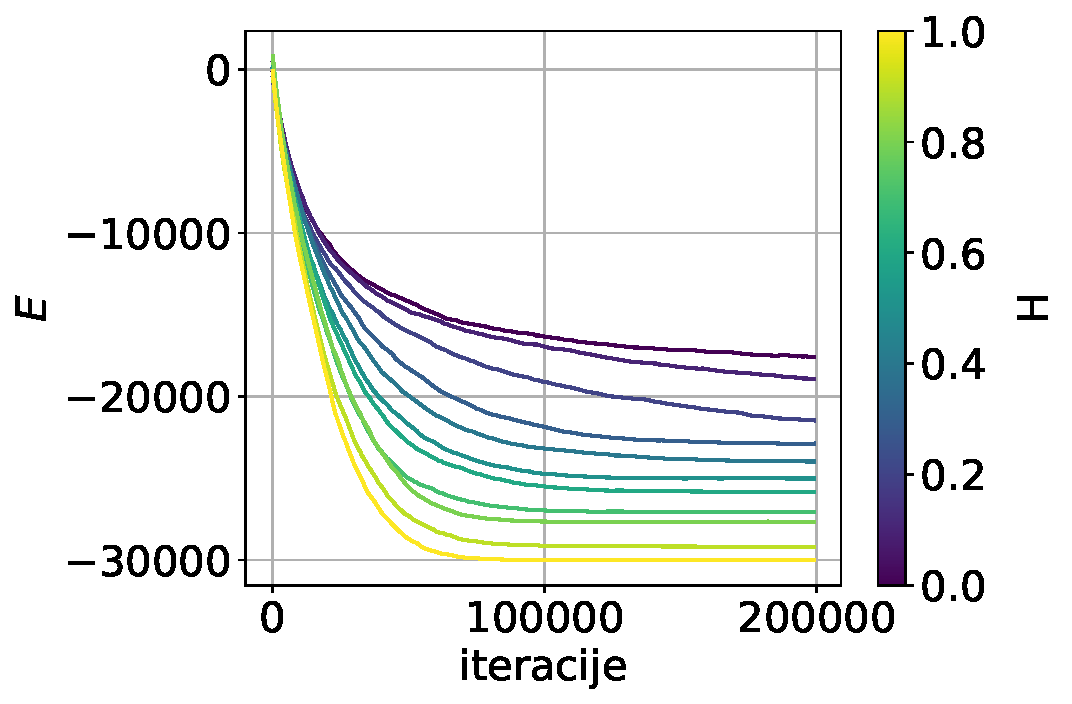
\includegraphics[width=\linewidth]{8.nal slike/metopolis_E_H.pdf}
        \caption[short]{Vpliv zunanjega polja na potek nižanja energije}
        \label{fig:E1}
    \end{minipage}
    \begin{minipage}{0.49\textwidth}
        \centering
        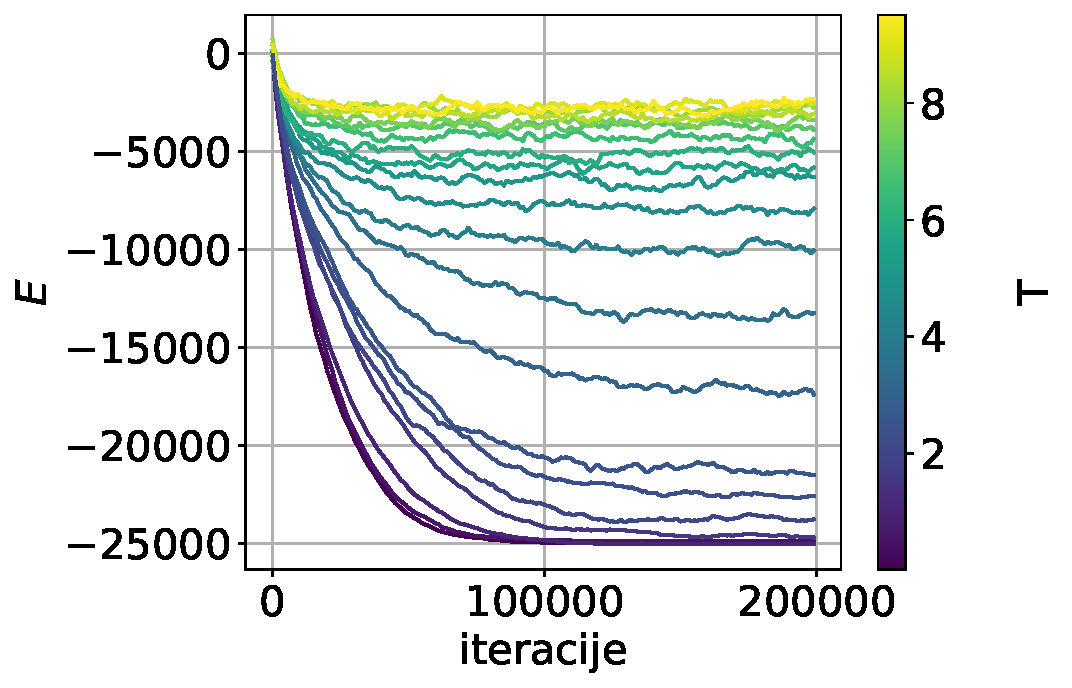
\includegraphics[width=\linewidth]{8.nal slike/metopolis_E_T.pdf}
        \caption[short]{Potek energije pri različnih temperaturah}
        \label{fig:E2}
    \end{minipage}\begin{minipage}{0.49\textwidth}
        \centering
        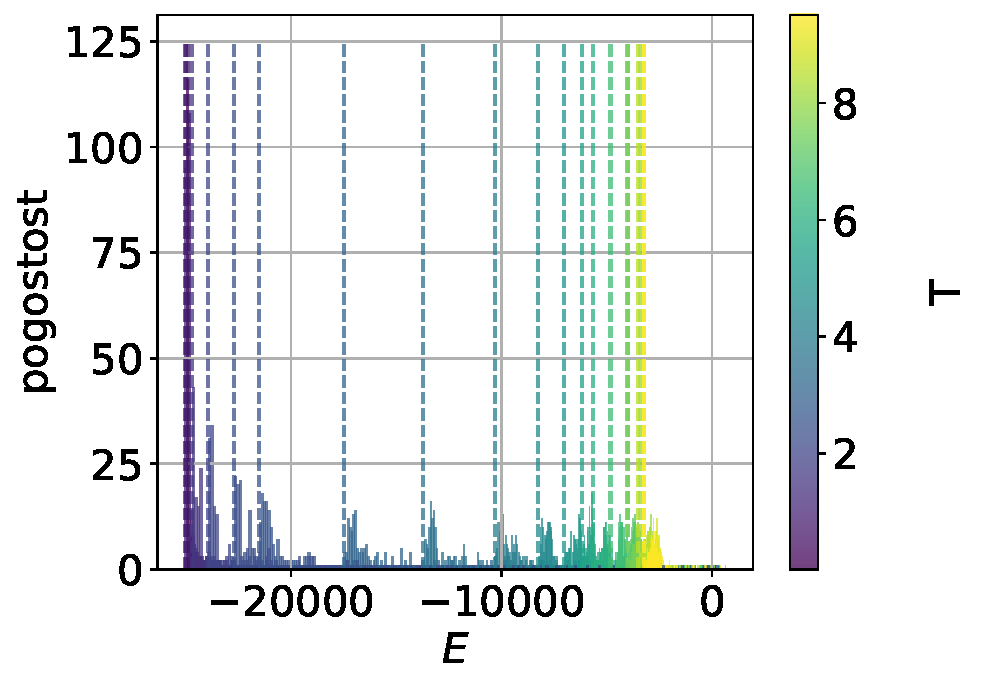
\includegraphics[width=\linewidth]{8.nal slike/metopolis_porazd_E.pdf}
        \caption[short]{Porazdeelitev pogostosti energije in označena najmanjša -- ravnovesna energija}
        \label{fig:E3}
    \end{minipage}
    \begin{minipage}{0.49\textwidth}
        \centering
        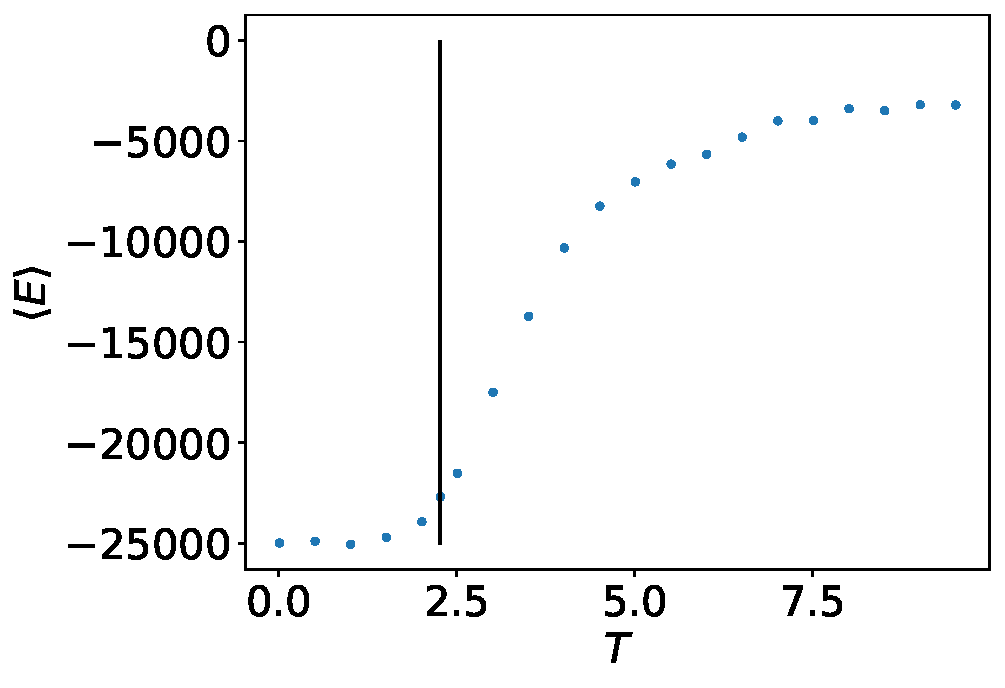
\includegraphics[width=\linewidth]{8.nal slike/metopolis_E_T_odv.pdf}
        \caption[short]{Odvisnosth ravnovesne energije od temperature}
        \label{fig:E4}
    \end{minipage}
\end{figure}

Na spodnjima slikama sta prikazana susceptibilnost in specifična toplota. Susceptibilnost je vedno pozitivna, kar je značilno za feromagnete. Verjetno lahko na obliko vplivamo tudi z zunanjim magnetnim poljem, vendar tega nismo poizkušali.
\begin{figure}[ht]
    \centering
    \begin{minipage}{0.45\textwidth}
        \centering
        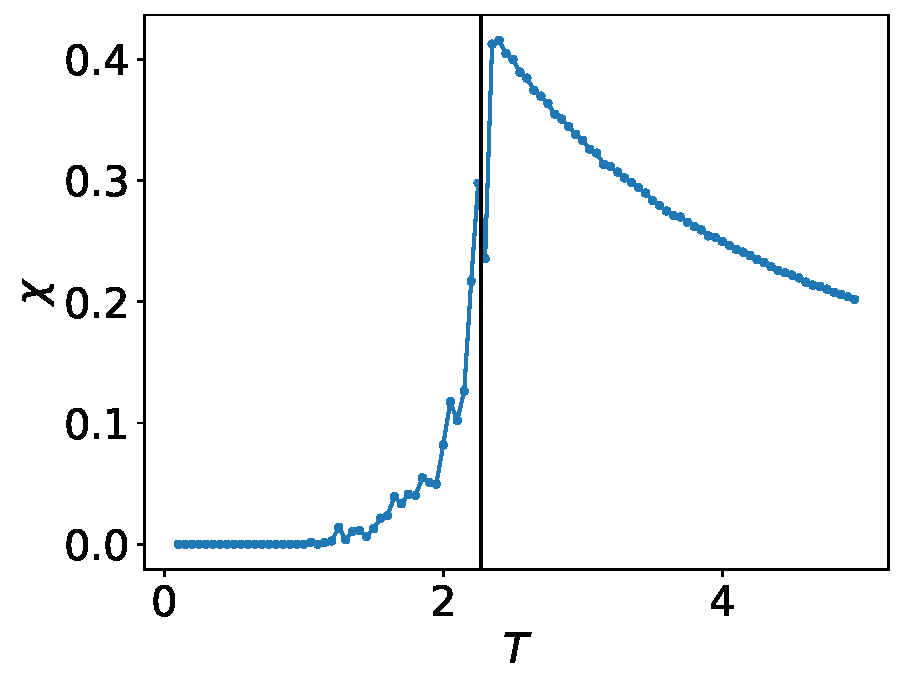
\includegraphics[width=\linewidth]{8.nal slike/suscept.pdf}
        \caption[short]{Susceptibilnost feromagneta v mreži 50x50, za 200 000 iteracij brez zunanjega polja}
    \end{minipage}
    \begin{minipage}{0.45\textwidth}
        \centering
        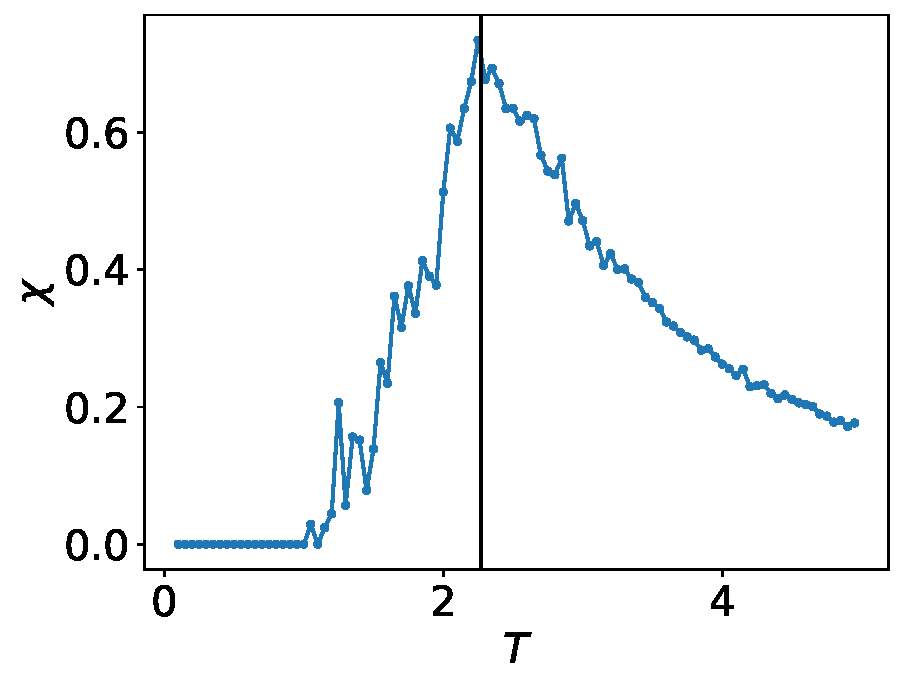
\includegraphics[width=\linewidth]{8.nal slike/kapac.pdf}
        \caption[short]{Specifična toplota feromagneta v mreži 50x50, za 200 000 iteracij brez zunanjega polja}
    \end{minipage}
\end{figure}

\subsection{Antiferomagnetizem}

Za antiferomagnete snovi velja $J=-1$. Zato take snovi ne težijo k ``enotnosti'', kot feromagneti, vendar se urejujejo v nasprotujoče si pare spinov +1 in -1 glede na sosede. Tudi tukaj je ta proces strukturiranja odvisen od temperature, kar je razvidno iz spodnjih slik. Pod temperaturo faznega prehoda je urejanje opazno, nad pa ne. Če bi pustili dovol iteracij, bi dosegli ravnovesno antiferomagnetno stanje, ko so vsi sosednji spini vsake opazovane točke ravno nasprotni. V tem primeru je razlika med robnima pogojema manj očitna, vendar vseeno raje uporabljamo periodične robne pogoje zaradi fizikalne pravilnosti in doseganja nižje (verjetno pravilnejše) ravnovesne energije. Opazimo tudi večja nihanja kot pri feromagnetih.
\begin{figure}[H]
    \centering
    \begin{minipage}{0.49\textwidth}
        \centering
        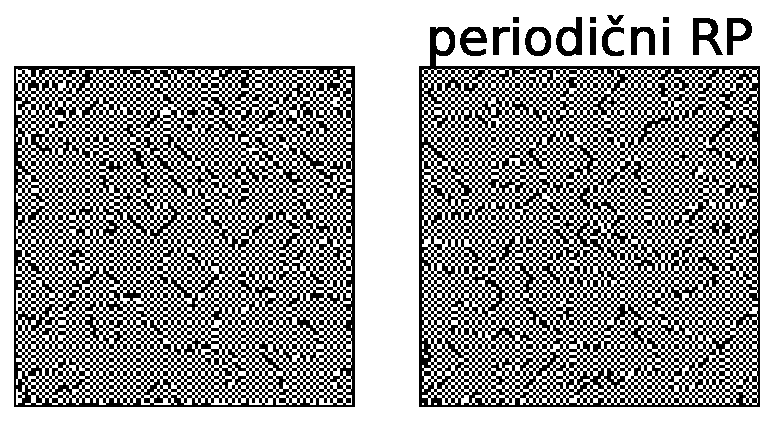
\includegraphics[width=\linewidth]{8.nal slike/metopolis_T_1_J.pdf}
        \caption[short]{$T=0.1$°C}
    \end{minipage}
    \begin{minipage}{0.49\textwidth}
        \centering
        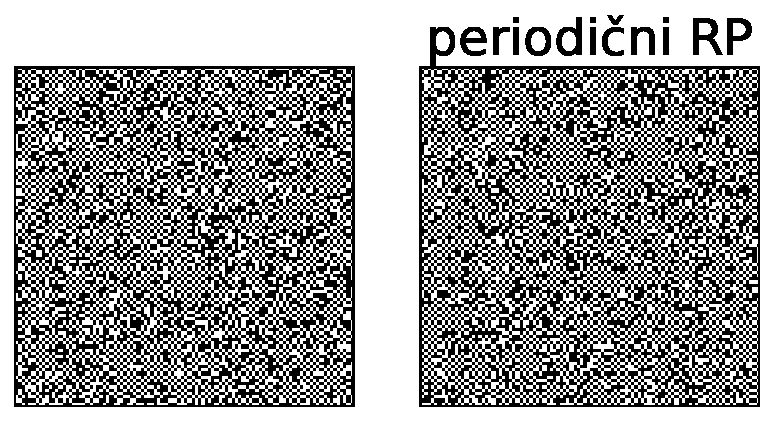
\includegraphics[width=\linewidth]{8.nal slike/metopolis_T_2.27_J.pdf}
        \caption[short]{$T=T_C=2.27$°C}
    \end{minipage}
    \begin{minipage}{0.49\textwidth}
        \centering
        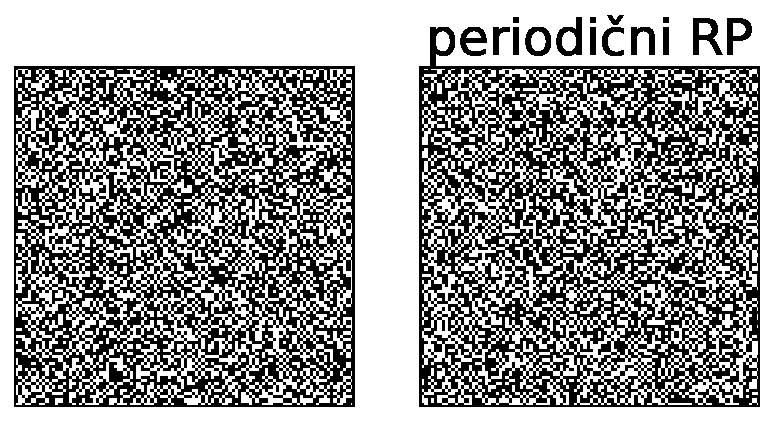
\includegraphics[width=\linewidth]{8.nal slike/metopolis_T_4_J.pdf}
        \caption[short]{$T=4.0$°C}
    \end{minipage}
    \begin{minipage}{0.45\textwidth}
        \centering
        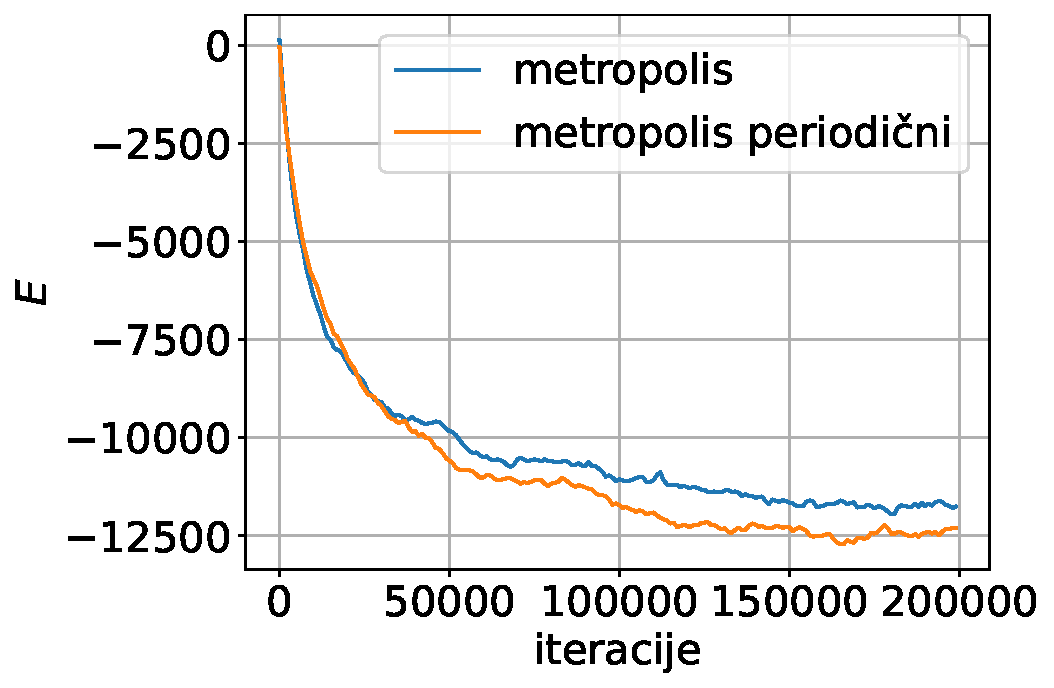
\includegraphics[width=\linewidth]{8.nal slike/metopolis_potek_E_J.pdf}
        \caption[short]{potek energije pri $T=2.27$°C}
    \end{minipage}
\end{figure}

Kar med fero- in antifero-magneti ni bistvenih razlik glede odvisnosti od temperature, izpuščamo večino prejšnjih grafov in prikazujemo le ta dva, ki izkazujeta bistvene lastnosti. To je neodvisnost antiferomagnetov od zunanjega magnetenega polja in odvisnost ravnovesne energije od temperature. Pri tem opazimo podobno globalno odvisnost kot pri feromagnetih, vendar tukaj prihaja tudi do minimalne energije pri $T=1$. Vzroka temu ne znamo najti, vendar se je to pojavilo večkrat in torej ni slučajen dogodek. 
\begin{figure}[ht]
    \centering
    \begin{minipage}{0.49\textwidth}
        \centering
        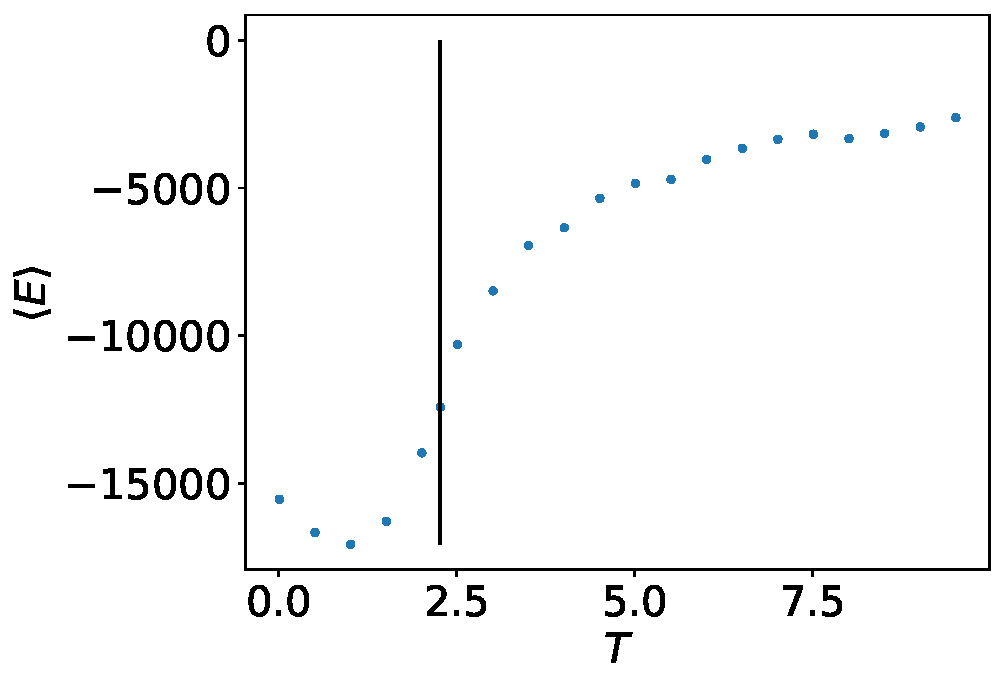
\includegraphics[width=\linewidth]{8.nal slike/metopolis_E_T_odv_J.pdf}
        \caption[short]{Odvisnosth ravnovesne energije od temperature za antiferomagnete}
    \end{minipage}
    \begin{minipage}{0.49\textwidth}
        \centering
        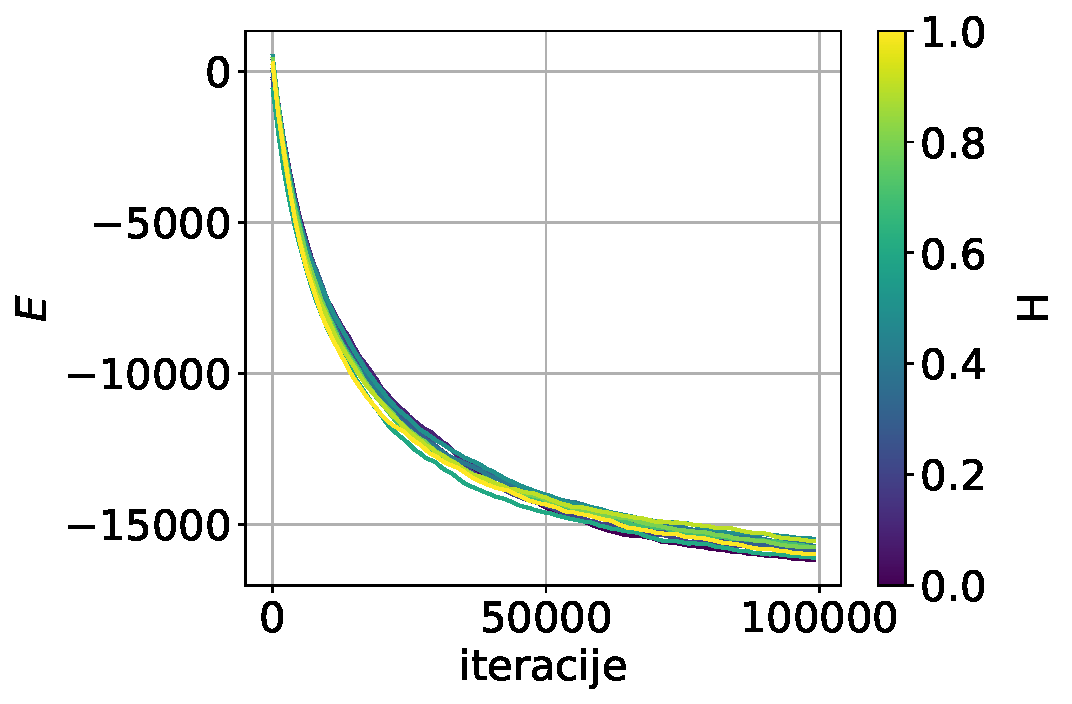
\includegraphics[width=\linewidth]{8.nal slike/metopolis_E_H_J.pdf}
        \caption[short]{Zunanje polje na antiferomagnete ne vpliva!}
    \end{minipage}
\end{figure}

Čeprav smo pričakovali, da bosta susceptibilnost in specifična toplota antiferomagneta različni od feromagnetne snovi, temu ni tako, vendar velja poudariti, da avtor za magnetno področje ni dobro podkovan.
\begin{figure}[ht]
    \centering
    \begin{minipage}{0.49\textwidth}
        \centering
        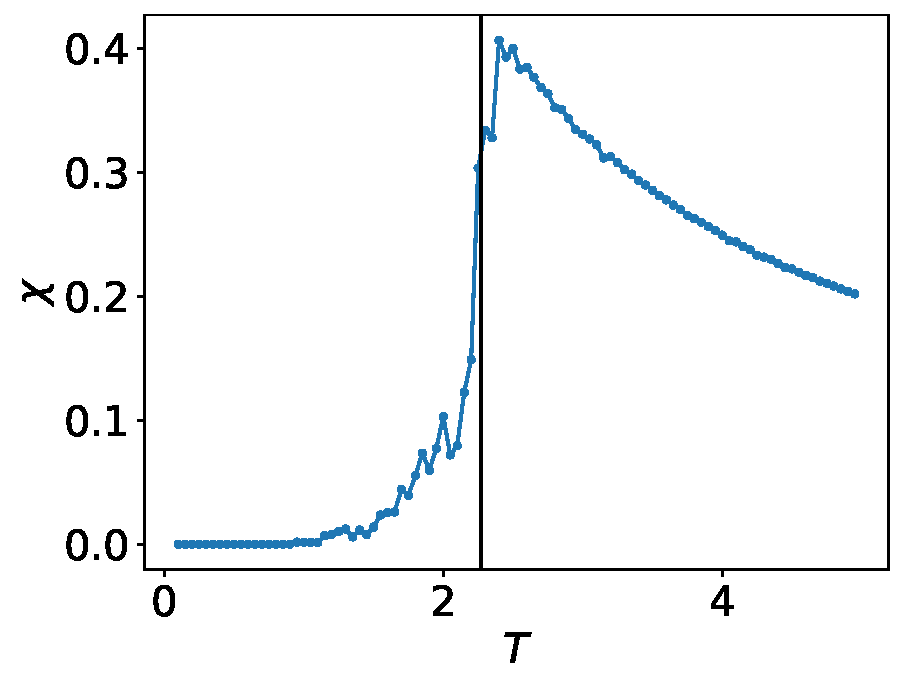
\includegraphics[width=\linewidth]{8.nal slike/sus_J.pdf}
        \caption[short]{Susceptibilnost antiferomagneta v mreži 50x50, za 200 000 iteracij brez zunanjega polja}
    \end{minipage}
    \begin{minipage}{0.49\textwidth}
        \centering
        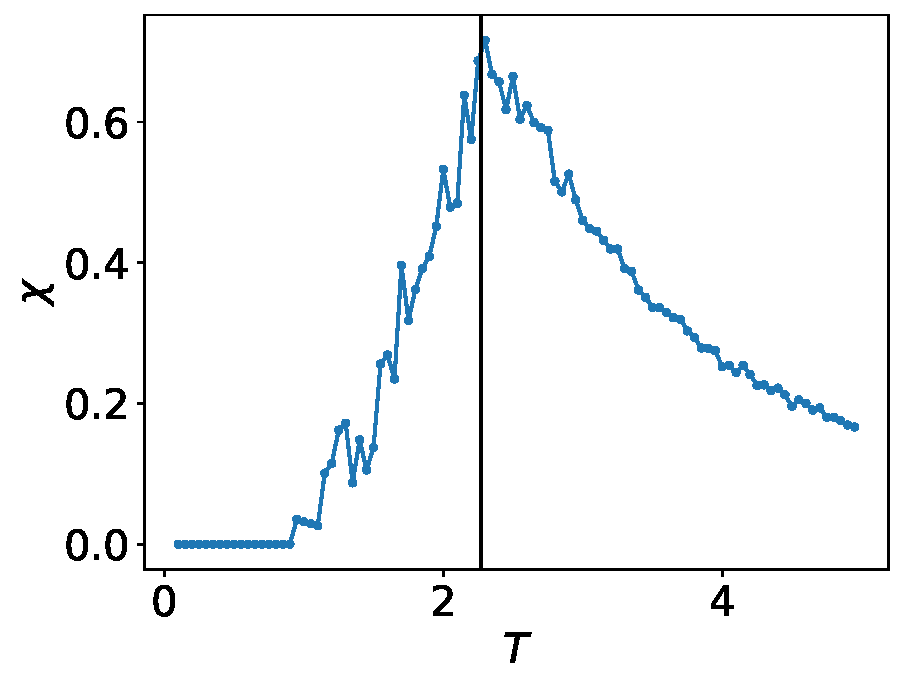
\includegraphics[width=\linewidth]{8.nal slike/kapac_J.pdf}
        \caption[short]{Specifična toplota antiferomagneta v mreži 50x50, za 200 000 iteracij brez zunanjega polja}
    \end{minipage}
\end{figure}